\documentclass[prd,10pt,superscriptaddress,notitlepage,tightenlines,nofootinbib,floatfix]{revtex4-1}
\usepackage{amssymb}   % for math
\usepackage{amsmath}
\usepackage{dsfont}
\usepackage{CJKutf8}   % for chinese names
\usepackage{graphicx}  % needed for figures
\usepackage{dcolumn}   % needed for some tables
\usepackage{bm}        % for math
\usepackage{xspace}
\usepackage{standalone}
\usepackage{enumitem}
%\usepackage[pdftex]{color}
\usepackage{color}
\usepackage{xcolor}
\usepackage{slashed}
\usepackage{booktabs}
\usepackage{multirow}
\usepackage{stackrel}
\usepackage{rotating}
\usepackage{pifont}
\usepackage{mathtools}
\usepackage{simplewick}
\usepackage{float} % Forces placement of figures
\usepackage{tikz} % adds /foreach (looping) command
\usepackage{hyperref}
\usepackage{subfigure} % subfigures
\hypersetup{
    colorlinks=true,       % false: boxed links; true: colored links
    linkcolor=blue,          % color of internal links
    citecolor=blue,        % color of links to bibliography
    filecolor=blue,      % color of file links
    urlcolor=blue           % color of external links
}


% Software
\def\chroma{\texttt{Chroma}\xspace}
\def\quda{\texttt{QUDA}\xspace}

% NEW COMMANDS
\def\note#1{\textbf{\color{red} COMMENT: #1}}
\def\andre#1{\textbf{\color{blue} ANDR\'E: {\color{red}#1}}}
\def\amy#1{\textbf{\color{purple} AMY: #1}}
\def\addcite#1{{\color{red}CITE[#1]}}
\def\new#1{{\color{blue}#1}}
% Refs
\def\eqref#1{{(\ref{#1})}}
\newcommand{\eqnref}[1]{Eq.~\eqref{#1}}
\newcommand{\Eqnref}[1]{Equation~\eqref{#1}}
\newcommand{\figref}[1]{Fig.~\ref{#1}}
\newcommand{\Figref}[1]{Figure~\ref{#1}}
\newcommand{\secref}[1]{Sec.~\ref{#1}}
\newcommand{\appref}[1]{App.~\ref{#1}}
% std for Table is to always use Table - strange
\newcommand{\tabref}[1]{Table~\ref{#1}}
\newcommand{\Tabref}[1]{Table~\ref{#1}}

% define colors
\newcommand{\red}[1]{{\color{red}{#1}}}
\newcommand{\blue}[1]{{\color{blue}{#1}}}

\definecolor{kngrey}{HTML}{A6AAA9}
\definecolor{knred}{HTML}{EC5D57}
\definecolor{knorange}{HTML}{F39019}
\definecolor{knyellow}{HTML}{F5D328}
\definecolor{kngreen}{HTML}{70BF41}
\definecolor{knblue}{HTML}{51A7F9}
\definecolor{knpurple}{HTML}{B36AE2}

\def\mc#1{{\mathcal #1}}
\def\ol#1{{\overline{#1}}}
\def\ket#1{{|#1\rangle}}
\def\bra#1{{\langle #1|}}

\DeclareMathOperator{\st}{str}
\DeclareMathOperator{\tr}{tr}
\DeclareMathOperator{\Erfc}{Erfc}
\DeclareMathOperator{\Erf}{Erf}
\DeclareMathOperator{\Tr}{Tr}

% Greek Letters
\def\a{{\alpha}}
\def\b{{\beta}}
\def\d{{\delta}}
\def\D{{\Delta}}
\def\e{{\epsilon}}
\def\g{{\gamma}}
\def\G{{\Gamma}}
\def\k{{\kappa}}
\def\l{{\lambda}}
\def\L{{\Lambda}}
\def\m{{\mu}}
\def\n{{\nu}}
\def\w{{\omega}}
\def\O{{\Omega}}
\def\S{{\Sigma}}
\def\s{{\sigma}}
\def\t{{\tau}}
\def\th{{\theta}}
\def\x{{\xi}}

%slash's
\def\Dslash{D\hskip-0.65em /}
\def\dslash{{\partial\hskip-0.5em /}}
\def\vslash{{\rlap \slash v}}
\def\qbar{{\overline q}}

% Jargon
\def\tsep{t_{\rm sep}}
\def\tinc{\tau_{\rm inc}}
\def\XPT{{$\chi$PT}}
\def\CPT{{$\chi$PT}}
\def\QCPT{{Q$\chi$PT}}
\def\PQCPT{{PQ$\chi$PT}}
\def\tr{\text{tr}}
\def\str{\text{str}}
\def\diag{\text{diag}}
\def\vit{{\it v}}
\def\vD{\vit\cdot D}
\def\tb{{\tilde b}}
\def\luscher{L{\"u}scher\xspace}



\begin{document}

\title{Bayes Model Averaging of the $D(p,\g)^3{\rm He}$ Reaction}


\author{Andr\'{e}~Walker-Loud}
\affiliation{Nuclear Science Division, Lawrence Berkeley National Laboratory, Berkeley, CA 94720, USA}
\email[]{walkloud@lbl.gov}

\date{\today}

\begin{abstract}
We perform a Bayes Model Averaging of two phenomenological descriptions and simple polynomial descriptions of the $S$-factor of the $D(p,\g)^3{\rm He}$ Reaction, also referred to as $S_{12}$.
This work was motivated by the INT Solar Fusion III Workshop, held in Berkeley, July 26-29, 2022, \url{https://indico.ice.csic.es/event/30/}.
\end{abstract}
\maketitle
\tableofcontents

\section{Results}
We have performed a Bayes Model Averaging of the $D(p,\g)^3{\rm He}$ $S$-factor, also known as $S_{12}$, using polynomials to various orders as well as a modification of the phenomenological prediction from Ref.~\cite{Marcucci:2005zc}.
The analysis strategy follows Ref.~\cite{Moscoso:2021xog} very closely.
What this work offers in addition is a Bayesian Model Averaging.
All results presented here can be reproduced utilizing the Python software provided at \url{https://github.com/walkloud/solar_fusion_reactions}.



The specific models considered are 
\begin{align}\label{eq:models}
S_{pheno}(E; a, b) &= a S_{nuc}(E) + b\, ,
\nonumber\\
S_{pheno}(E; a) &= a S_{nuc}(E)\, ,
\nonumber\\
S_{poly}^{(n)}(E; S_i) &= \sum_{i=0}^n S_i E^i\, ,
\end{align}
for $n=2,3,4,5$ and $S_{nuc}(E)$ is an update of that in Ref.~\cite{Marcucci:2005zc} provided by L.~Marcucci.
The model averaging is performed using an approximation of the Bayes Factor determined in the limit that all distributions can be approximated as Gaussian.

We consider two model averages, one utilizing all models in Eq.~\eqref{eq:models} and one using only the polynomial models.  The reason for considering these two averages is that we do not have good prior information as to whether the two $S_{pheno}(E)$ models are reasonable given the extracted values of $a$.
Details of the analysis are presented in Sec.~\ref{sec:S_12_bma}, following a general discussion of Bayes Model Averaging in Sec.~\ref{sec:bma}.




\subsection{All models}
Using the Gaussian Bayes Factors from the analysis, the $S_{pheno}(E;\lambda)$ models are strongly favored over the polynomial models.
The models used and their resulting log Gaussian Bayes Factors (logGBF), relative weigths, augmented $\chi^2_{aug}/dof$ and $Q$ values are presented in Table~\ref{tab:all_models}.
From this analysis, the model average $S$ factor at two different energies is given by
\begin{align}\label{eq:all_models}
S_{12}(E=0) &= 2.028(51)(09)\times10^{-7} \textrm{ MeV b}\, ,
\nonumber\\
S_{12}(E=91{\rm keV}) &= 8.11(16)(00)\times10^{-7} \textrm{ MeV b}\, ,
\end{align}
where the first uncertainty is the weighted statistical uncertainty and the second uncertainty arises from the model variance.
The model average posterior distributions for the full $S$-factor, as well as these two kinematic points are presented in Fig.~\ref{fig:all_models}.

\begin{table}
\begin{ruledtabular}
\begin{tabular}{rclcc}
model& logGBF& weight& $\chi_{aug}^2/dof[dof]$& Q\\
\hline
$S_{pheno}(E; a)$       & 1478.7 & 0.585    & 0.7659[96] & 0.957\\
$S_{pheno}(E; a, b)$    & 1478.3 & 0.414    & 0.7629[96] & 0.960\\
$S_{poly}^{(3)}(E; S_i)$& 1470.2 & 1.21e-04 & 0.6988[96] & 0.989\\
$S_{poly}^{(4)}(E; S_i)$& 1469.2 & 4.62e-05 & 0.6946[96] & 0.990\\
$S_{poly}^{(5)}(E; S_i)$& 1468.2 & 1.63e-05 & 0.6934[96] & 0.990\\
$S_{poly}^{(2)}(E; S_i)$& 1464.1 & 2.86e-07 & 0.8541[96] & 0.845\\
\end{tabular}
\end{ruledtabular}
\caption{\label{tab:all_models}
The logGBF and relative weights of the various models.
}
\end{table}


\begin{figure}
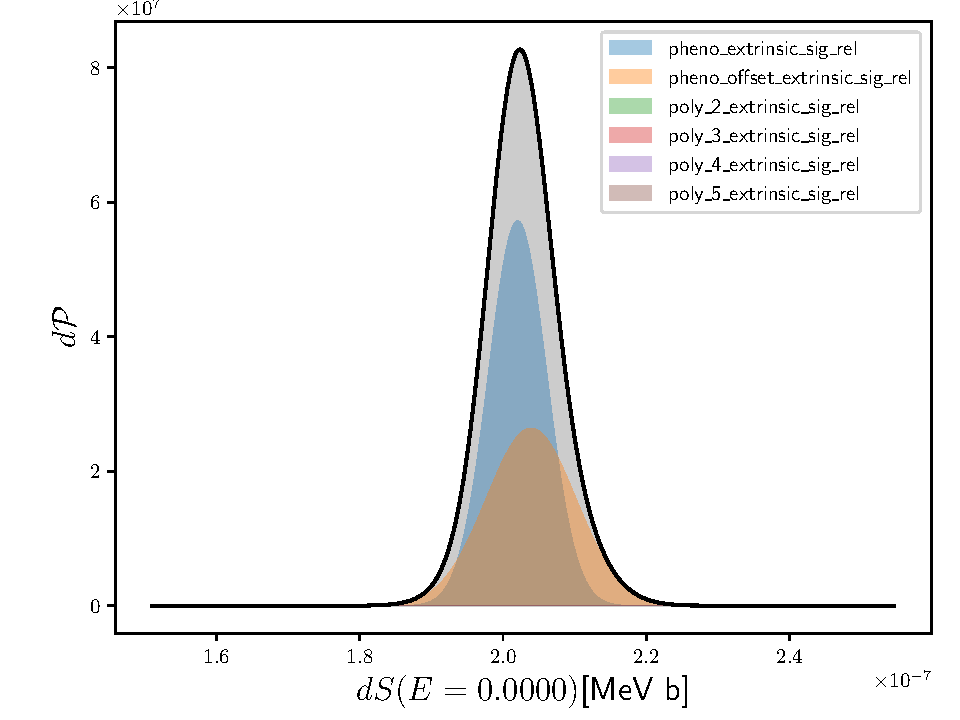
\includegraphics[width=0.48\textwidth]{figures/S_E0.0000_hist_all}
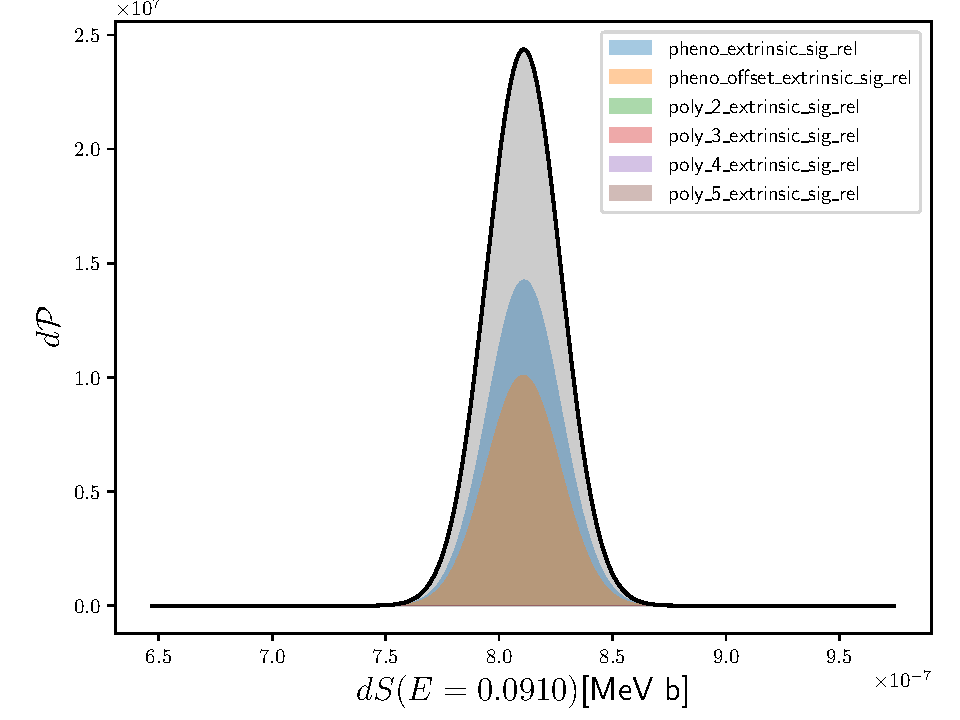
\includegraphics[width=0.48\textwidth]{figures/S_E0.0910_hist_all}
\caption{\label{fig:all_models}
The model average $S$-factor versus energy compared with the data as well as the weighted distributions at $E=0$ and $E=91$~keV.}
\end{figure}

A potential issue with this model average is that the scale factors, $a$, of the $S_{pheno}(E)$ models is determined to be
\begin{align}
&a = 0.921(19)& &\textrm{ for $S_{pheno}(E; a)$}\, ,&
\nonumber\\
&a = 0.918(20)& &\textrm{ for $S_{pheno}(E; a,b)$}\, ,&
\end{align}
which implies that in both cases, the phenomenological prediction $S_{nuc}(E)$ is to large by approximately 8\%.
Is it reasonable to expect that this prediciton could be wrong by 8\%?




\subsection{Polynomial models only}

We also present the Bayes Model Average considering only the polynomial fit functions.
These result in model average $S$-factor of
\begin{align}
S_{12}(E=0) &= 2.088(89)(05)\times10^{-7} \textrm{ MeV b}\, ,
\nonumber\\
S_{12}(E=91{\rm keV}) &= 7.99(18)(00)\times10^{-7} \textrm{ MeV b}\, ,
\end{align}
The model weights are presented in table~\ref{tab:poly} and the model average fit is presented in \figref{fig:poly}.
At the $1-\s$ level, these results are consistent with those in \eqnref{eq:all_models}.

\begin{table}
\begin{ruledtabular}
\begin{tabular}{rclcc}
model& logGBF& weight& $\chi_{aug}^2/dof[dof]$& Q\\
\hline
$S_{poly}^{(3)}(E; S_i)$& 1470.2 & 0.658 & 0.6988[96] & 0.989\\
$S_{poly}^{(4)}(E; S_i)$& 1469.2 & 0.252 & 0.6946[96] & 0.990\\
$S_{poly}^{(5)}(E; S_i)$& 1468.2 & 0.089 & 0.6934[96] & 0.990\\
$S_{poly}^{(2)}(E; S_i)$& 1464.1 & 1.56e-03 & 0.8541[96] & 0.845\\
\end{tabular}
\end{ruledtabular}
\caption{\label{tab:poly}
The logGBF and relative weights of the various models when only polynomials are considered.
}
\end{table}
    
\begin{figure}
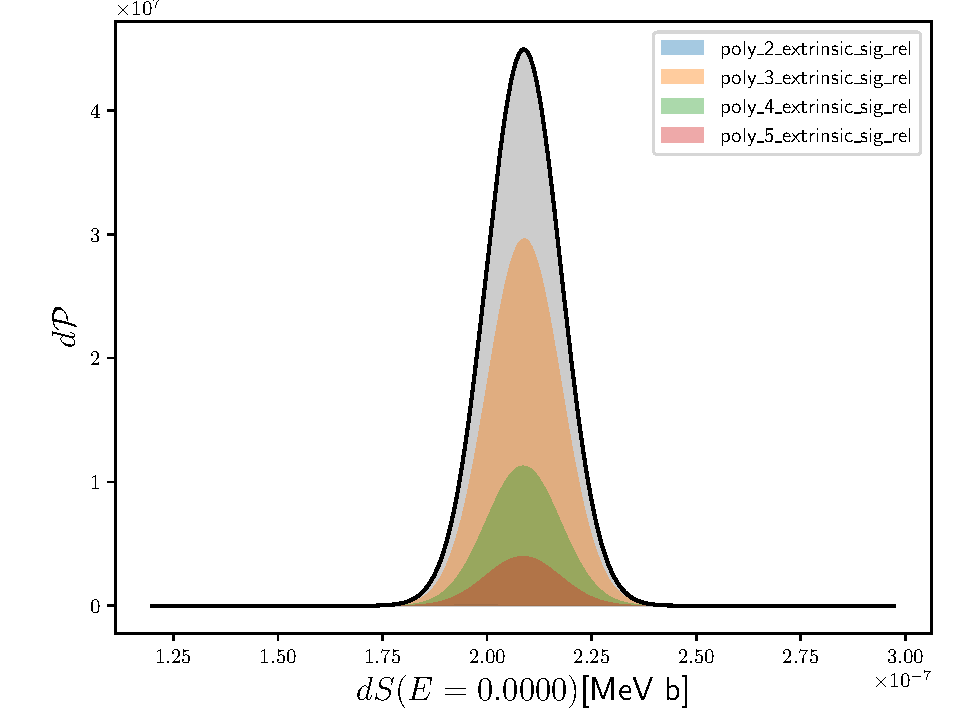
\includegraphics[width=0.48\textwidth]{figures/S_E0.0000_hist_poly}
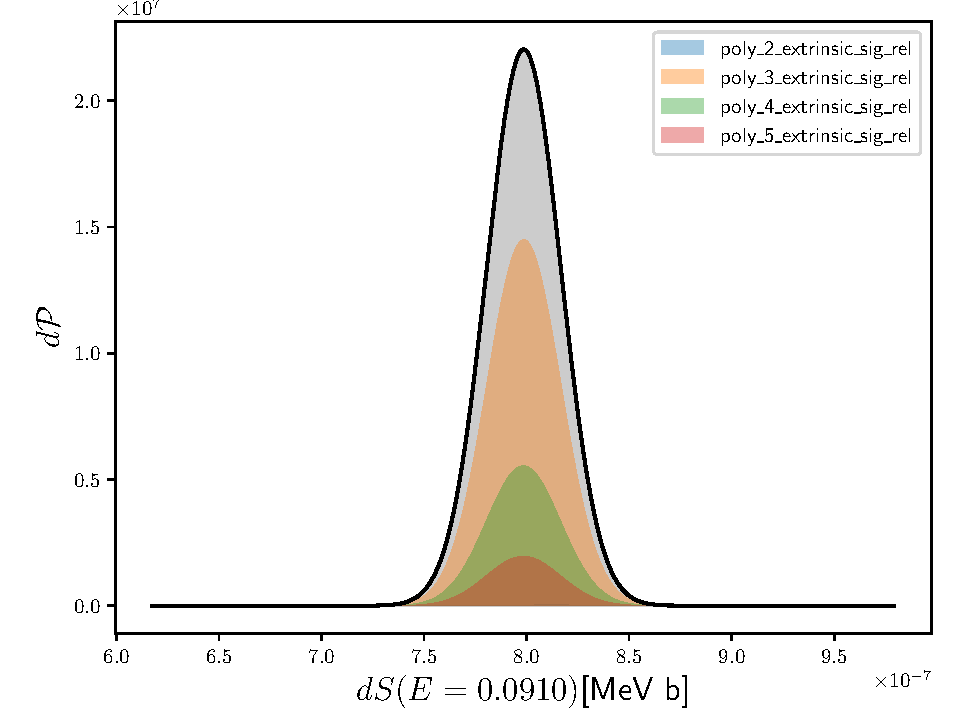
\includegraphics[width=0.48\textwidth]{figures/S_E0.0910_hist_poly}
\caption{\label{fig:poly}
The polynomial only model average $S$-factor versus energy compared with the data as well as the weighted distributions at $E=0$ and $E=91$~keV.}
\end{figure}


\begin{figure}
\begin{tabular}{cc}
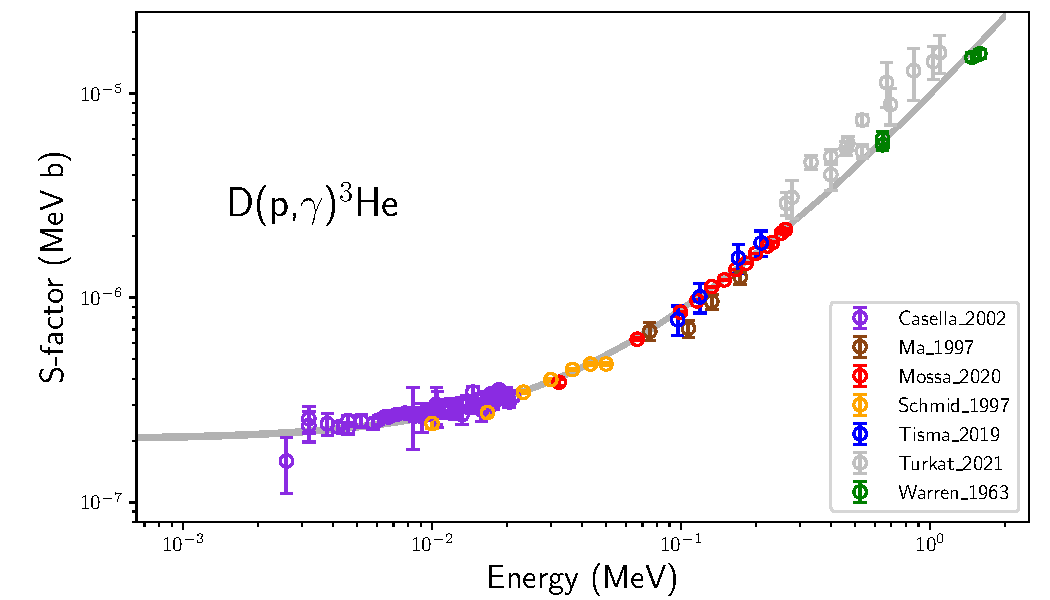
\includegraphics[width=0.49\textwidth]{figures/S_model_avg_all}
&
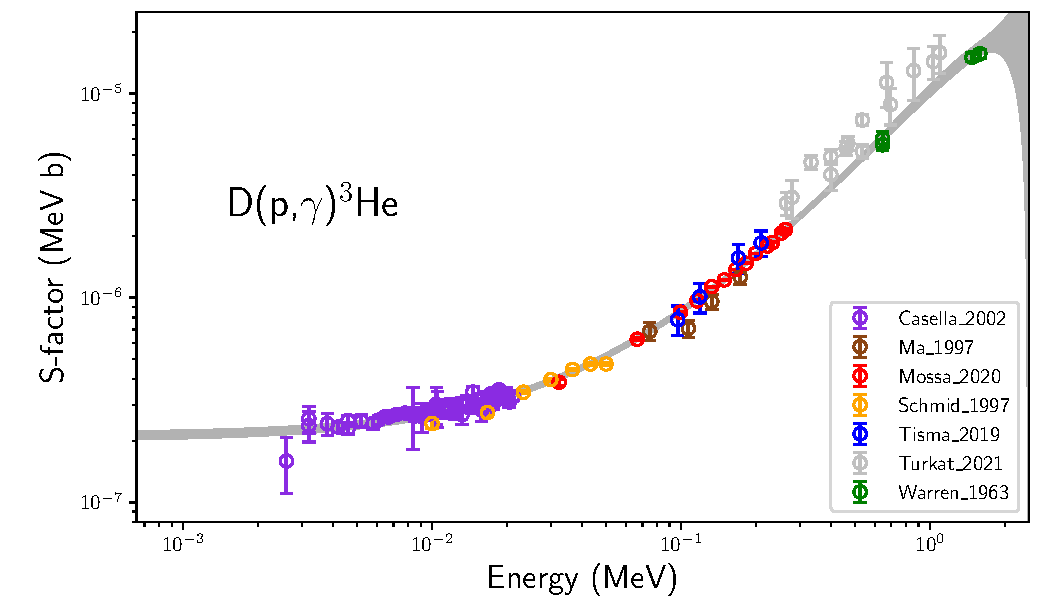
\includegraphics[width=0.49\textwidth]{figures/S_model_avg_poly}
\\
(all models) & (polynomial)
\end{tabular}
\caption{\label{fig:S_factor_E}
The $S$-factor versus energy compared with the data as well as the weighted distributions at $E=0$ and $E=91$~keV.}
\end{figure}
    



\section{Motivation}

The starting point for this work is Ref.~\cite{Moscoso:2021xog}, which provided a detailed Bayesian analysis of $S_{12}$ using a phenomenology inspired prediction as well as a third order polynomial in energy.
The phenomenology prediction was taken from Ref.~\cite{Marcucci:2005zc}, 
and is referred to as $S_{nuc}$ in Ref.~\cite{Moscoso:2021xog}. 
This $S_{nuc}$ prediction was determined using the AV18 and UIX phenomenological potentials for two and three-body nucleon interactions, respectively.
In order to fit the results, this prediction was multiplied by a scale factor and an offset was added.
The two functions to describe $S(E)$ were then
\begin{align}
S_{pheno} &= a S_{nuc}(E) + b\, ,
\nonumber\\
S_{poly} &= S_0 + S_1 E + S_2 E^2 + S_3 E^3\, .
\end{align}
There are a few important issues that were described in Ref.~\cite{Moscoso:2021xog}, which we will describe.
What this work adds in addition to Ref.~\cite{Moscoso:2021xog} is a Bayesian Model Averaging procedure to enable a weighted average over several models.

Specifically, we consider the same $S_{pheno}$ function as above, but also a variant where the offset is not included.  We further consider polynomial descriptions of $\mathrm{O}(E^2)$ through $\mathrm{O}(E^5)$.
By utilizing Bayes Theorem, we can construct a relative weight for each model, given the data.  In the absence of any prior information preferring one model over another, we can then perform a model averaging using the weights derived from Bayes Theorem.

All results presented here can be reproduced by installing and running the code availabe at \url{https://github.com/walkloud/solar_fusion_reactions}.
This is a lightweight Python package that can perform the analysis of $S_{12}$.  It was designed with the idea that, if useful, additional reactions could also be supported.


\section{Bayes Model Averaging in general \label{sec:bma}}

We use Gaussian priors for all parameters, such that the objective function which is minimized to determine the posterior distributions of all parameters is given by
\begin{equation}
\chi^2_{aug} = \sum_d \left( \frac{y_d - f(x_d;\l)}{\s_d}\right)^2 
    + \sum_i \left( \frac{\l_i - \tilde{\mu}_i}{\tilde{\s}_i} \right)^2\, ,
\end{equation}
where in this observable, all the data $y_d$ are deteremined with uncorrelated uncertainties $\s_d$.
The user choses a prior mean $\tilde{\mu}_i$ and width $\tilde{\s}_i$ for each parameter $\l_i$ that is being deteremined in the analysis.





Using Bayes' Theorem, we can ask conditional probabilities, such as what is the probability distribution of a given observable, given the data, which we can obtain by ``marginalizing'' over the space of models that describe the observable.  For example, the posterior distribution of the $S$-factor can be determined with 
\begin{equation}
P(S | D) = \int d\l P(S | M(\l), D) P(M(\l) | D)\, ,
\end{equation}
where $\l$ is a parameter that spans the space of both, what model is used, as well as the continuous parameters upon which the model depends upon.
In this expression, $P(S | M(\l), D)$ is the posterior likelihood distribution of our observable $S$, given a particular model $M(\l)$ and the data $D$.
$P(M(\l) | D)$ is the posterior likelihood distribution of the model given the data, and through Bayes' theorem, we can relate this to the likelihood that the data is given by a particular model, 
\begin{equation}
P(M(\l)|D) = \frac{P(D|M(\l)) P(M(\l))}{\int d\l P(D|M(\l))P(M(\l))}\, .
\end{equation}

In practice, the marginialization over models is carried out by utilizing a finite number of models, such that the integrals are replaced with sums:
\begin{align}
P(S|D) &\simeq \sum_k P(S|M_k, D) P(M_k|D)\, ,
\nonumber\\
P(M_k|D) &\simeq \frac{P(D|M_k) P(M_k)}{\sum_j P(D|M_j) P(M_j)}\, .
\end{align}
If the probability of the data given a model, $P(D|M_k)$, is determined by marginalizing over the paramters of the model
\begin{equation}
P(D|M_k) = \int \prod_j d\theta_j^{(k)} P(D|\theta_j^{(k)}, M_k) P(\theta_j^{(k)}|M_k)\, ,
\end{equation}
then $P(D|M_k)$ is a number which can be interpreted as a relative weight for model $k$.
In practice, we can approximate this marginalization by finding the values of the parameters that maximize the Bayes Factor, which is equivalent to maximinzing the probability of a given model with respect to the priors for the parameters.  Explicit examples of this prior optimization will be presented in Sec.~\ref{sec:prior_optimization}.

Without prior information, one assumption that can be made is to assume each model is equally likely, a uniform distribution of models, which leads to a simple weighting procedure.  This is the simplest to implement, and the least subject to physicist bias.  This would be as close to a purely data-drive approach as possible.  On the other hand, we might have significant prior reasons to favor or disfavor certain classes of models.  This will be explored in Sec.~\ref{sec:s_12_bma}.


\section{Bayes Model Averaging of $S_{12}$ \label{sec:S_12_bma}}

Before discussing the model averaging, we first summarize the important issues described in Ref.~\cite{Moscoso:2021xog} for fitting the $S_{12}$ $S$-factor data.


\subsection{Prior Optimization \label{sec:prior_optimization}}

Without prior knowledge about the size of unknown parameters of a model, one of the trickiest things in building a constrained Bayesian fit can be chosing the priors, both their distribution as well as the mean values and widths used to constrain the priors.

The approach we take to this problem is to use normal (Gaussian) priors, and then use the (Gaussian) Bayes Factors (GBF) as a relative weight that can be used to optimize the otherwise unknown priors.
One advantage of this approach is that, in the limit all the distributions can be approximated by Gaussians, the Bayes Factor can be approximated by the GBF and computed analytically.  See this discussion in the 
\href{https://lsqfit.readthedocs.io/en/latest/overview.html?highlight=Bayes%20Factor#correlated-parameters-gaussian-bayes-factor}{lsqfit readthedocs}.

In order to elucidate this process, let us consider the 3rd order polynomial parameterization of the $S$-factor
\begin{equation}
    S_3(E) = S_0 + S_1 E + S_2 E^2 + S_3 E^3\, .
\end{equation}
By looking at the data, we can guess a prior for $S_0$ to be $\tilde{S}_0 = N(2\times10^{-7}, 1\times10^{-7})$, which means a normal distribution with mean $\mu=2\times10^{-7}$ and width $\s=1\times10^{-7}$.  We have chosen a prior width that we expect to be very large compared to what would be obtained in a fit, such that the prior has minimal influence on the posterior distribution of this parameter.

Similarly, we may like the data to provide the constraint on $S_1$, so we also can give a large prior width.  Thinking about the higher order coefficients, it becomes less clear, without processing the data somehow, to have an intuition for the natural size of these terms.  We could undertake a human-expensive trial and error search for good paramters, or, we can use the GBF parameters for a fit, with a chosen value of the prior widths, to let the data inform us what the optimal choice of prior width is.

In Fig.~\ref{fig:poly_3_prior}, we plot the relative weight of a model of $S_3(E)$ where the different models are specified by the width of the prior of the $S_3$ parameter.  Specifically, we have chosen
\begin{align}\label{eq:poly_priors}
&\tilde{S}_0 = 10^{-7}\times N(2,1)\, ,&
&\tilde{S}_1 = 10^{-5}\times N(0,1)\, ,&
&\tilde{S}_2 = 10^{-5}\times N(0,1)\, ,&
&\tilde{S}_3 = 10^{-6}\times N(0, \tilde{\s})\, ,&
\end{align}
and then we perform a bunch of fits, varying the parameter $\tilde{\s}$, from each fit, compute the GBF, and then use these to compte the relative weigth of each model,
\begin{equation}
w_k = \frac{e^{{\rm logGBF}_k}}{\sum_l e^{{\rm logGBF}_l}}\, .
\end{equation}
From the figure, we see that a value of $\tilde{\s}\approx5\times10^{-6}$ gives the largest GBF, and thus the largest relative weight.
We could chose to marginalize over $\tilde{\s}$ by summing the product of the relative weight times the model, for each choice of the parameter.
In practice, if we pick a value of $\tilde{\s}$ that is close to that which maximizes the GFB, this is most often sufficient to capture the relative weight of a given model function as compared to other model functions: choosing $\tilde{\s} = 4\times10^{-6}$, $5\times10^{-6}$ or $6\times10^{-6}$ will have very little effect on the relative weight of $S_3(E)$ as compared to $S_2(E)$ or $S_4(E)$ or other models.

\begin{figure}
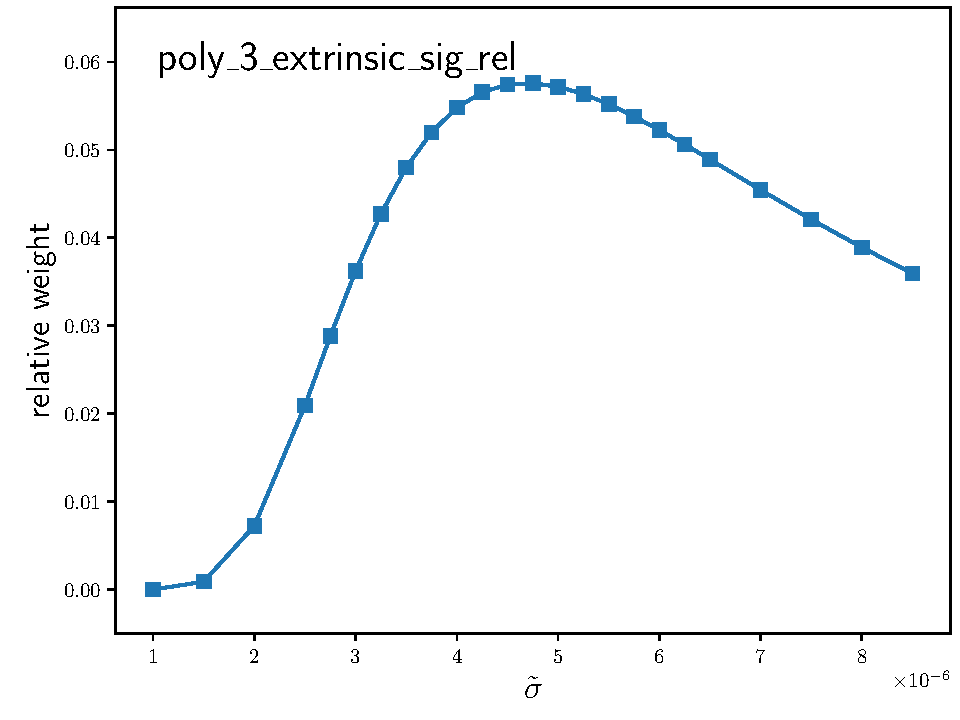
\includegraphics[width=0.48\textwidth]{figures/poly_3_extrinsic_sig_rel_prior_width_study}
\caption{\label{fig:poly_3_prior}
Relative weight of $S_3(E)$ versus the prior width on the coefficient of the $E^3$ order term.
The relative weight is determined from the ratio of the GBF from a particular choice of $\tilde{\s}$ to the sum over the GBF factors from all choices of $\tilde{\s}$.  A value of $\tilde{\s}\approx5\times10^{-6}$ optimizes the GBF, and thus has the highest weight.}
\end{figure}


In Fig.~\ref{fig:poly_prior}, we show a similar prior-width optimization for the parameters $S_3$, $S_4$ and $S_5$ (when used) in the second, fourht and fifth order polynomial model functions.  In all cases, the priors of $S_0$, $S_1$ and $S_2$ are chosen as in Eq.~\eqref{eq:poly_priors}, and then the prior widths of all higher order coefficients are set to $N(0,\tilde{\s})$ and the GBF is determined with a simultaneous variation of this coefficient for all higher order priors together.
Varying these parameters together is just to simplify the search for the optimal widths, without doing a grid search in the widths of the different priors being optimized.  Such a strategy is also good because it helps prevent a user from over-optmiizing the priors.
We observe that in all cases, a prior width of $\tilde{\s}=4\times10^{-6}$ is near the value that maximizes the GBF.
In the subsequent model averaging, we fix the prior widths of the various polynomial coefficients of order $n\geq3$ with this value and the other prior widths are chosen as in Eq.~\eqref{eq:poly_priors}.

The one clear enhancement over the study presented here would be to make the polynomial function as 
\begin{equation}
    S_n = \sum_{i=0}^n S_i \left(\frac{E}{E_{ref}}\right)^i\, ,
\end{equation}
where $E_{ref}$ is some reference energy scale (chosen by the user), such that all the coefficients are dimensionless.

\begin{figure}
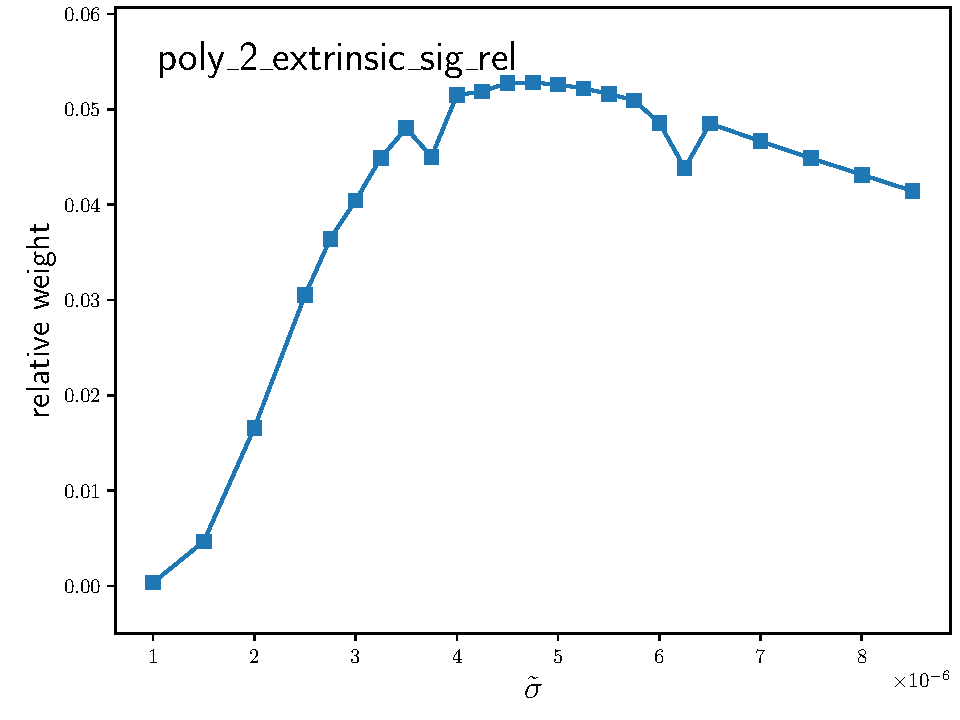
\includegraphics[width=0.32\textwidth]{figures/poly_2_extrinsic_sig_rel_prior_width_study}
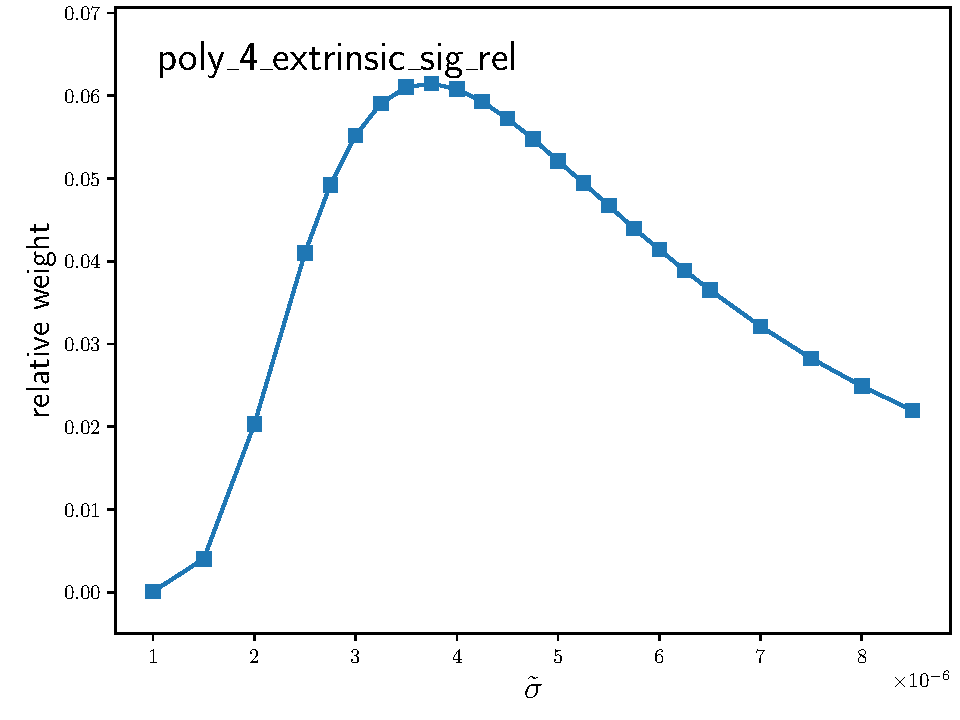
\includegraphics[width=0.32\textwidth]{figures/poly_4_extrinsic_sig_rel_prior_width_study}
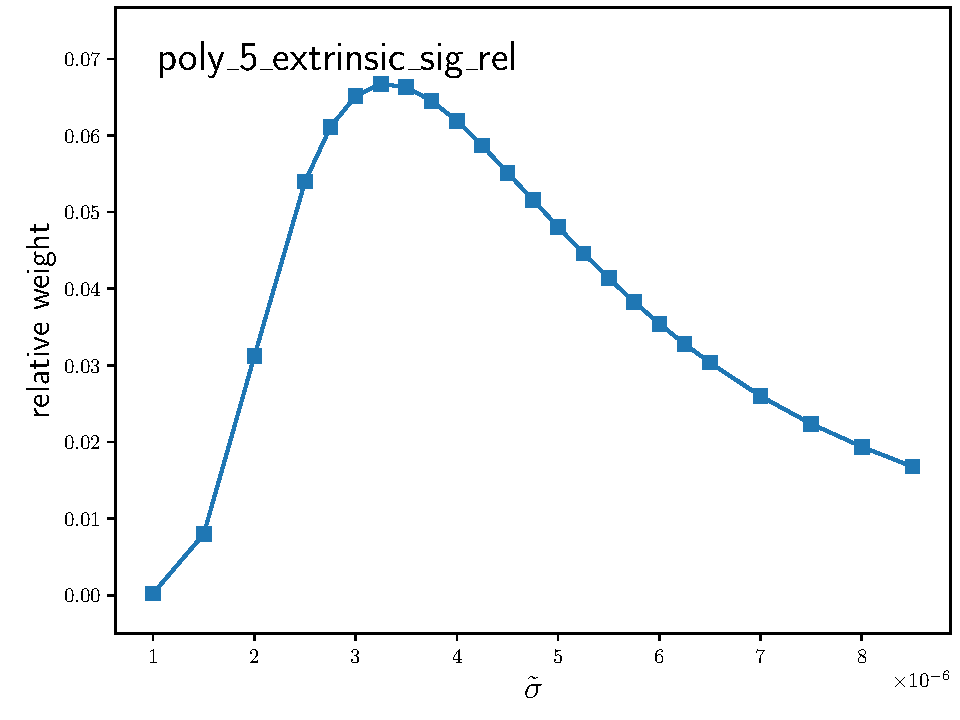
\includegraphics[width=0.32\textwidth]{figures/poly_5_extrinsic_sig_rel_prior_width_study}
\caption{\label{fig:poly_prior}
Relative weight of various order polynomial fit functions as a function of the prior width, as described in the text.}
\end{figure}


In \figref{fig:scale_factor_width}, we show a similar study using the phenomenological fit function, $S_{pheno}(E;a)$ and varying the prior width on the scale factor, $a$.

\begin{figure}
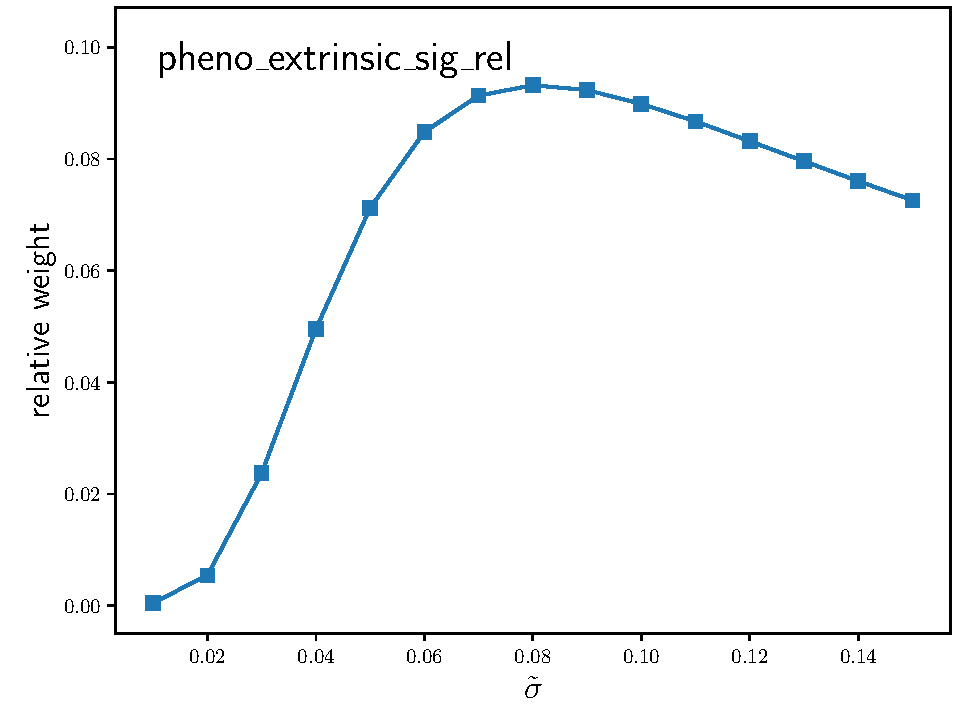
\includegraphics[width=0.48\textwidth]{figures/pheno_extrinsic_sig_rel_prior_width_study}
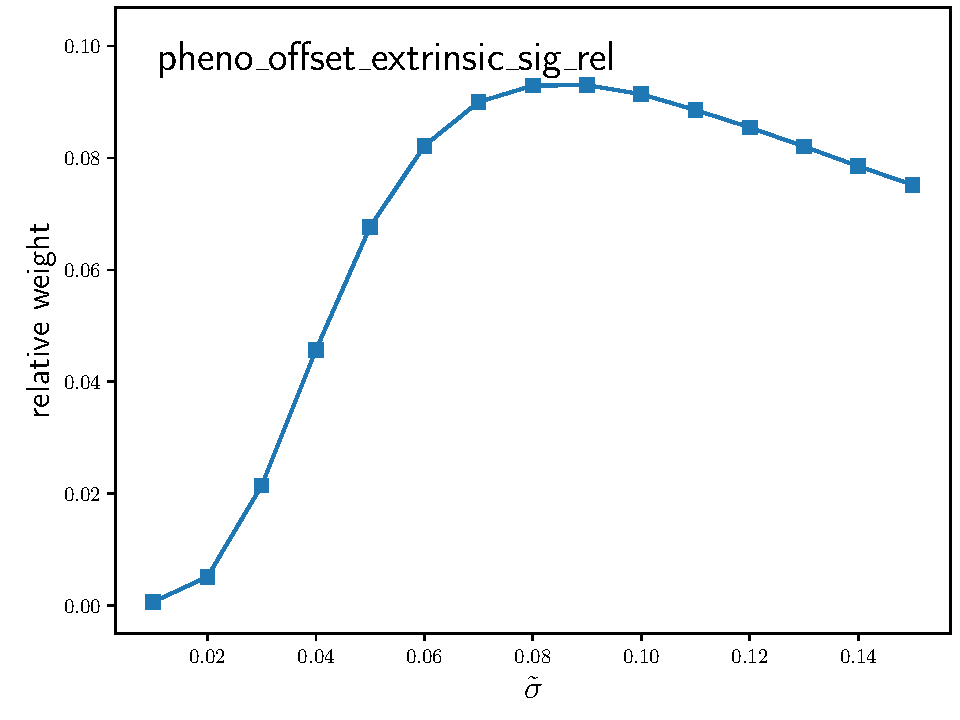
\includegraphics[width=0.48\textwidth]{figures/pheno_offset_extrinsic_sig_rel_prior_width_study}
\caption{\label{fig:scale_factor_width}
Relative weight of $S_{pheno}(E;a)$ (left) and $S_{pheno}(E;a,b)$ (right) as a function of the prior width of the scale factor, $a$.}
\end{figure}


\subsection{$S_{12}$ model average \label{sec:s_12_bma}}

As described in Ref.~\cite{Moscoso:2021xog}, there are two modifications to a standard least-squares optimization that we undertake for the analysis.
The first is to use a log-normal normalization factor for each dataset to treat the systematic uncertainties.
The second is to add an unknown, extrinsic stochastic uncertainty to each dataset.  Quoting Ref.~\cite{Moscoso:2021xog}:
\quote{In many cases, the observed scatter of the measured data cannot be explained solely by the reported statistical uncertainties, suggesting the presence of additional sources of statistical uncertainties unknown to the experimenter.  We utilize the expression extrinsic uncertainty for describing such effects~\cite{deSouza:2019pmr}.}
These extrinsic uncertainties can be added for each data set as an absolute, energy-independent correction, as in Ref.~\cite{Moscoso:2021xog}, or they can be added as relative to the mean value of $S(E)$, as in Ref.~\cite{Odell:2021tqd}.
We explore both options.

\begin{verbatim}
# relative extrinsic uncertainty
z_cutoff = 1.

for dset in dsets:
    dy_extrinsic = y[dset].mean  *  z_cutoff * arctan(z[dset]**2 / z_cutoff)
    y_prime      = y + normal(0, dy_extrinsic)

# absolute extrinsic uncertainty
for dset in dsets:
    dy_extrinsic = z_cutoff * arctan(z[dset]**2 / z_cutoff)
    y_prime      = y + normal(0, dy_extrinsic)
\end{verbatim}
In both cases, the parameters \texttt{z[dset]} are not known ahead of time and they are determined by optimizing the Bayes Factor, as described in Sec.~\ref{sec:prior_optimization}, using the \href{https://lsqfit.readthedocs.io/en/latest/lsqfit.html?highlight=empbayes#lsqfit.empbayes_fit}{lsqfit.empbayes} function taking as input \texttt{y\_prime} for the data, as described in the \href{https://lsqfit.readthedocs.io/en/latest/overview.html?highlight=unknown#y-has-unknown-errors}{y has Unknown Errors} of the \href{https://lsqfit.readthedocs.io/}{lsqfit.readthedocs}.
We note that the objects \texttt{y} and \texttt{y\_prime} are Gaussian Variables, from the \href{https://github.com/gplepage/gvar}{gvar} Python package, which treats the objects as Gaussian random variables, tracking the error propagation when using them with arithmatic expressions.

Then, the fit is performed by finding values of the parameters which minimize the augmented $\chi^2$ function defined by
\begin{equation}
\chi^2_{aug} = \sum_{d} \sum_{i_d} 
    \frac{\big( y_{d,i_d} - f_d \times S(E; \lambda) \big)^2}{\s_{d,i_d}^2 + (\s_d^{ext})^2}
    +\sum_p \left( \frac{\l_p - \tilde{\mu}_p}{\tilde{\s}_p} \right)^2\, .
\end{equation}
The sum over $d$ is a sum over the various datasets used in the analysis.
The sum over $i_d$ is a sum over the uncorrelated data samples, $y_{d,i_d}$ in each dataset with quoted statistical uncertainty $\s_{d,i_d}$.
For each dataset, the fit function is multiplied by a log-normal normalization factor $f_d$, given by the quoted systematic uncertainty from the original publication of the data.
The inverse, $1/f_d$, is a factor one would multiply the data by to bring it in line with the resulting fit function at the optimized values of the parameters.
For each dataset, an unknown statistical extrinsic uncertainty $\s_d^{ext}$ is added, which is determined in the analysis.

The analysis can be performed turning on and off many of these features using the fitting code \url{https://github.com/walkloud/solar_fusion_reactions}.
Here we present results for two fits as examples:
\begin{verbatim}
    -----------------------------------------------------------
    pheno_extrinsic_sig_rel
    -----------------------------------------------------------
    Least Square Fit:
      chi2/dof [dof] = 0.77 [96]    Q = 0.96    logGBF = 1478.7
    
    Parameters:            posterior      [ prior      ]  *-sigma tension
                      a    0.921 (19)     [ 1.000 (80) ]
     log(f_Turkat_2021)    0.284 (46)     [  0.00 (13) ]  **
      log(f_Mossa_2020)   -0.014 (20)     [ 0.000 (27) ]
      log(f_Tisma_2019)    0.009 (63)     [ 0.000 (95) ]
    log(f_Casella_2002)    0.040 (21)     [ 0.000 (44) ]
     log(f_Schmid_1997)   -0.037 (28)     [ 0.000 (86) ]
         log(f_Ma_1997)   -0.122 (43)     [ 0.000 (86) ]  *
     log(f_Warren_1963)   -0.072 (33)     [ 0.000 (95) ]
    ----------------------------------------------------
          f_Turkat_2021    1.329 (61)     [  1.00 (13) ]  **
           f_Mossa_2020    0.986 (20)     [ 1.000 (27) ]
           f_Tisma_2019    1.009 (63)     [ 1.000 (95) ]
         f_Casella_2002    1.041 (22)     [ 1.000 (44) ]
          f_Schmid_1997    0.964 (27)     [ 1.000 (86) ]
              f_Ma_1997    0.885 (38)     [ 1.000 (86) ]  *
          f_Warren_1963    0.930 (31)     [ 1.000 (95) ]
    
    Settings:
      svdcut/n = 1e-12/0    tol = (1e-08,1e-10,1e-10*)    (itns/time = 6/0.0)
      fitter = scipy_least_squares    method = trf
    
\end{verbatim}
\begin{verbatim}
    -----------------------------------------------------------
    poly_3_extrinsic_sig_rel
    -----------------------------------------------------------
    Least Square Fit:
      chi2/dof [dof] = 0.7 [96]    Q = 0.99    logGBF = 1470.2
    
    Parameters:
                    S_0   2.089(89)e-07      [ 2.0(1.0)e-07 ]
                    S_1    5.92(25)e-06      [ 0.0(1.0)e-05 ]
                    S_2    6.34(88)e-06      [ 0.0(1.0)e-05 ]
                    S_3   -2.25(54)e-06      [ 0.0(4.0)e-06 ]
                      a      1.000 (80)      [   1.000 (80) ]
     log(f_Turkat_2021)      0.265 (49)      [    0.00 (13) ]  **
      log(f_Mossa_2020)     -0.002 (22)      [   0.000 (27) ]
      log(f_Tisma_2019)      0.018 (63)      [   0.000 (95) ]
    log(f_Casella_2002)      0.024 (30)      [   0.000 (44) ]
     log(f_Schmid_1997)     -0.040 (31)      [   0.000 (86) ]
         log(f_Ma_1997)     -0.111 (43)      [   0.000 (86) ]  *
     log(f_Warren_1963)     -0.048 (54)      [   0.000 (95) ]
    ---------------------------------------------------------
          f_Turkat_2021      1.303 (64)      [    1.00 (13) ]  **
           f_Mossa_2020      0.998 (22)      [   1.000 (27) ]
           f_Tisma_2019      1.018 (64)      [   1.000 (95) ]
         f_Casella_2002      1.025 (30)      [   1.000 (44) ]
          f_Schmid_1997      0.961 (30)      [   1.000 (86) ]
              f_Ma_1997      0.895 (38)      [   1.000 (86) ]  *
          f_Warren_1963      0.953 (51)      [   1.000 (95) ]
    
    Settings:
      svdcut/n = 1e-12/0    tol = (1e-08,1e-10,1e-10*)    (itns/time = 7/0.0)
      fitter = scipy_least_squares    method = trf
    
\end{verbatim}



\bibliography{sf_refs}



%%%%%%%%%%%%%%%%%%%%%%%%%%%%%%%%%
%%%%%%%%%%%%%%%%%%%%%%%%%%%%%%%%%
%%%%%%%%%%%%%%%%%%%%%%%%%%%%%%%%%

\end{document}

